\chapter{Popis navrženého řešení}

V předešlé kapitole byla vysvětlena základní problematika, která souvisí s virtualizací síťových funkcí, cloud computingem a softwarově definovanými sítěmi. Zároveň byla popsána referenční architektura frameworku pro virtualizaci síťových funkcí. Tato kapitola bude již věnována konkrétnímu příkladu využití virtuálních síťových funkcí v cloudovém prostředí. Bude zde popsána navržená architektura pro privátní cloudovou platformu využívající virtualizaci síťových funkcí, kterou mohou využívat všichni její uživatelé. Pro tuto cloudovou platformu a pro její uživatele byli navrženy dva příklady virtuálních síťových funkcí. U obou příkladů jsou uvedeny scénáře, způsob jakým jsou navrženy a způsob jakým mohou uživatelé tyto virtuální síťově funkce spravovat.

\section{Architektura navrženého řešení}

Architektura navrženého řešení vychází z referenční architektury popsané v kapitole \ref{sub:architektura}. Jak je vidět na obrázku č. \ref{fig:VNF_overview}


\begin{figure}[h]
\begin{centering}
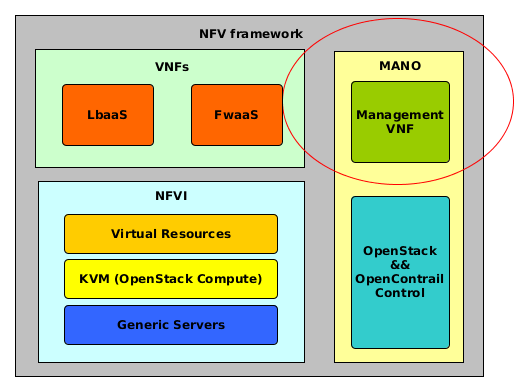
\includegraphics[scale=0.51]{images/VNF_overview}
\par\end{centering}
\caption{Architektura NFV řešení\label{fig:VNF_overview}}
\end{figure}


\subsection{OpenStack}\label{sub:interaction}

Popis Openstacku

OpenStack Heat Templates are used to demonstrate load balancing and firewalling inside of Openstack.

\subsection{OpenContrail}\label{sub:interaction}

Popis OpenContrailu.


\section{Firewall as a Service}


\subsection{Scénář NAT}

\subsection{Scénář Service Chaining}

\subsection{Scénář HA firewall}


\section{Load balancer as a Service}

Popis funkce load balanceru v 


\section{Heat Templates}



\begin{figure}[h]
\begin{centering}
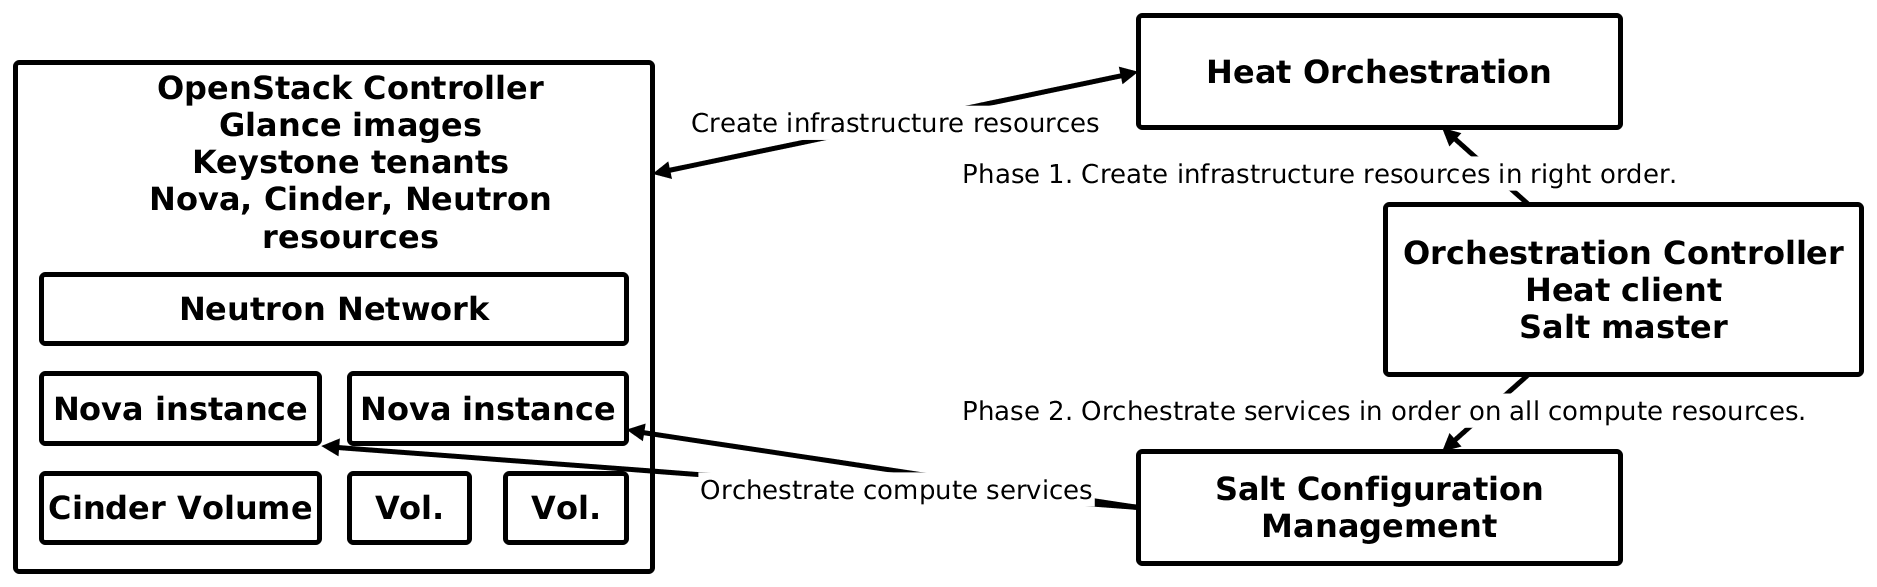
\includegraphics[scale=0.21]{images/heat}
\par\end{centering}
\caption{Popis heat orchestrace\label{fig:heat}}
\end{figure}

Popis co jsou to heat templates.

Heat is the main project of the OpenStack orchestration program. It allows users to describe deployments of complex cloud applications in text files called templates. These templates are then parsed and executed by the Heat engine.

\subsection{FwaaS template}

Pro FwaaS je narhnut heat template, který obsahuje:

\begin{itemize}
\item 1 firewall instanci
\item 1 testovaci instanci
\item 1 management instanci
\item management síť
\item privátní síť
\item contrail policy
\end{itemize}



\subsection{LbaaS template}


Navržený heat template pro LbaaS v sobě obsahuje následující prostředky, které se po spuštění pokusí vytvořit.

\begin{itemize}
\item pool
\item members
\item health monitoring
\item 2 web instance
\item privatni síť
\item public síť
\end{itemize}
